\documentclass[11pt, onecolumn, oneside, reqno]{article}
\usepackage[english]{babel}
\usepackage{geometry}                		% See geometry.pdf to learn the layout options. There are lots.
\geometry{a4paper}
%\geometry{landscape}                		% Activate for rotated page geometry
\usepackage[parfill]{parskip}
\usepackage{graphicx} % Use pdf, png, jpg, or eps§ with pdflatex; use eps in DVI mode, TeX will automatically convert eps --> pdf in pdflatex		
\usepackage{amsmath, mathtools}  
%\usepackage{bbm}              %$\mathbbm{Q}$
%\usepackage{mathrsfs}         %$\mathscr{L}$
\usepackage{apacite}
\usepackage{caption} 
%\captionsetup[table]{skip=100pt}
\usepackage{abstract}

%\usepackage[colorlinks=true,	urlcolor=blue,	linkcolor=green]{hyperref}

\title{Udacity Kinematics Project: Pick \& Place}
\author{Stephan Hohne}
\date{June 29, 2017}

\begin{document}
\maketitle

\begin{abstract}
This document contains supporting material for my solution of the \emph{Pick \& Place} kinematics project, which is part of the Robotics Nanodegree by Udacity. In the first section I summarize basic trigonometry which is used for describing the kinematics of a robotic arm. Then I describe the Denavit-Hartenberg conventions for assigning reference frames to robotic manipulators. The third sections contains design data for the KUKA KR210 robotic arm.
\end{abstract}

\tableofcontents

\listoftables

\newpage

\section{Geometry}
\subsection{Euler Rotations}
The goal is to find the Euler angles $\alpha$, $\beta$ and $\gamma$ for a given three dimensional rotation which is represented by a $3 \times 3$ matrix with nine elements,
\begin{equation}
R_z \left(\alpha \right) \, R_y \left(\beta \right) \, R_x \left(\gamma \right) =
\begin{pmatrix}
r_{11} & r_{12} & r_{13} \\
r_{21} & r_{22} & r_{23} \\
r_{31} & r_{32} & r_{33}
\end{pmatrix} \, .
\end{equation}
Then the Euler angles are defined as
\begin{eqnarray}
\alpha & = & \arctan \left( \frac{r_{21}}{r_{11}} \right) \, , \\
\beta & = & \arctan \left( \frac{-r_{31}}{\sqrt{r_{11}^2 + r_{21}^2}} \right) \, , \\
\gamma & = & \arctan \left( \frac{r_{32}}{r_{33}} \right) \, .
\end{eqnarray}
We follow the convention where $\alpha$ is the yaw angle around the $z$-axis, $\beta$ is the pitch around the $y$-axis and $\gamma$ is the roll around the $x$-axis.

\section{Robot Kinematics}
\subsection{Denavit-Hartenberg Parameters}
In 1955, Jacques Denavit and Richard Hartenberg proposed a systematic method of attaching reference frames to the links of a manipulator that simplified the homogeneous transforms. Their method only requires four parameters to describe the position and orientation of neighboring reference frames.

The convention described here is consistent with \cite{Craig-2005}. We denote the Cartesian base for frame $i$ as $\hat{x}_i$, $\hat{y}_i$ ,  $\hat{z}_i$.

We assign a reference frame to each link so that the frame moves rigidly with the link. We choose $\hat{x}_{i-1}$ so that is normal to the plane spanned by $\hat{z}_{i-1}$ and $\hat{z}_i$. The resulting vector can be determined using the cross product as
\begin{equation}
\label{eq:common_normal}
\hat{x}_{i-1}^{\pm} = \pm \frac{\hat{z}_{i-1} \times \hat{z}_i}{\begin{Vmatrix}
\hat{z}_{i-1} \times \hat{z}_i
\end{Vmatrix}} \, .
\end{equation}

The transformation between frame $i-1$ and frame $i$ is then characterized by four parameters.
\begin{itemize}
\item The twist angle $\alpha_{i-1}$ is the angle between $\hat{z}_{i-1}$ and $\hat{z}_i$ measured in a right hand sense about $\hat{x}_{i-1}$.
\item The link length $a_{i-1}$ is the distance from $\hat{z}_{i-1}$ to $\hat{z}_i$ measured along $\hat{x}_{i-1}$. Beware as this is not always equal to the actual length of the link.
\item The link offset $d_i$ is the signed distance from $\hat{x}_{i-1}$ to $\hat{x}_i$ measured along $\hat{z}_i$. This quantity is variable for a prismatic joint.
\item The joint angle $\theta_i$ is the angle between $\hat{x}_{i-1}$ and $\hat{x}_i$ measured in a right hand sense about $\hat{z}_{i-1}$. This quantity is variable for a revolute joint.
\end{itemize}

The parameter assignment process for open kinematic chains with $n$ degrees of freedom  is summarized as, The assignment algorithm is as follows.
\begin{enumerate}
\item Assign labels $\left\lbrace 0, \ldots , n\right\rbrace$ to links and $\left\lbrace 1, \ldots , n\right\rbrace$ to joints, starting with the fixed base link.
\item Draw lines through all joints, defining the joint axes.
\item Assign the $Z$ axis of each frame to point along its joint axis.
\item Identify the common normal between the $Z$ axes of subsequent frames according to equation \ref{eq:common_normal}.
\item The endpoints of intermediate links (i.e. not the base link or the end effector) are associated with the two joint axes $j$ and $j+1$. For frames $j = 1, \ldots n$ choose the base vectors $\hat{x}_j$ as follows.
\begin{itemize}
\item For skew axes, along the normal between $\hat{z}_j$ and $\hat{z}_{j+1}$. Choose the sign so that $\hat{x}_j$ points from frame $j$ to $j+1$.
\item For intersecting axes, normal to the plane containing $\hat{z}_j$ and $\hat{z}_{j+1}$.
\item For parallel or coincident axes, the assignment is arbitrary. Look for ways to make other DH parameters equal to zero.
\end{itemize}
\item For the base link, always choose frame 0 to be coincident with frame 1 when the first joint variable $\theta_1$ or $d_1$ is equal to zero. This will guarantee that $\alpha_0 = a_0 = 0$. If joint 1 is revolute then $d_1 = 0$. If joint 1 is prismatic then $\theta_1 = 0$.
\item For the end effector frame, if joint $n$ is revolute, choose $\hat{x}_n$ to be in the direction of $\hat{x}_{n-1}$ for $\theta_n = 0$. Choose the origin of frame $n$ such that $d_n = 0$.
\end{enumerate}

Special cases involving the $Z$ axes are
\begin{itemize}
\item collinear lines: $\alpha = a = 0$
\item parallel lines: $\alpha = 0$, $a \neq 0$
\item intersecting lines: $\alpha \neq 0$, $a = 0$
\item If the common normal intersects the $Z$ axis of frame $i$ at the origin, then $d_i = 0$.
\end{itemize}

To keep track of the values of these parameters while constructing the reference frames, we write them down in a table. Once the frame assignments are made, the DH parameters are typically presented in tabular form. Each row in the table corresponds to the transform from frame $i$ to frame $i+1$.

\subsection{Homogeneous Transformations}
The concepts of rotations, translations, and homogeneous transforms are essential to understanding the forward kinematics problem of manipulators: given the joint variables, calculate the location of the end effector. The solution procedure involves attaching a reference frame to each link of the manipulator and writing the homogeneous transforms from the fixed base link to the subsequent links, all the way to the end effector.  The resulting transformation is then the matrix product of the transformations. For a robot with $n + 1$ links $\left\lbrace 0, \ldots , n\right\rbrace$ this is a product over the $n$ joints,
\begin{equation}
\prescript{0}{n} T = \prod_{i = 1}^n
\prescript{i-1}{i} T
\end{equation}

The homogeneous transform from frame $i-1$ to frame $i$ is composed of a sequence of four basic transformations, two rotations $R$ and two translations $D$,
\begin{equation}
\prescript{i-1}{i} T =
R \left(X_{i-1} , \alpha_{i-1}\right) D \left(X_{i-1} , a_{i-1}\right)
R \left( Z_i , \theta_i\right) D_Z \left( Z_i , d_i\right) \, .
\end{equation}
The corresponding homogeneous transform matrix is of the form 
\begin{equation}
\prescript{i-1}{i} T =
\begin{pmatrix}
c \theta_i & -s\theta_i & 0 & a_{i-1} \\
s \theta_i \, c \alpha_{i-1} & c \theta_i \, c \alpha_{i-1} & -s \alpha_{i-1} & -s \alpha_{i-1} d_i \\
s \theta_i \, s \alpha_{i-1} & c \theta_i \, s \alpha_{i-1} &  c \alpha_{i-1} & c \alpha_{i-1} d_i \\
0 & 0 & 0 & 1
\end{pmatrix} \, .
\end{equation}

Given the DH parameters, either as constant values provided by the robot design, or variables determined by the current robot pose we can then read off the pose of the end effector from the overall transformation matrix $\prescript{0}{n} T$. The location in Cartesian coordinates and the orientation in Euler angles.

\subsection{Inverse Kinematics for a Spherical Wrist}
This section follows lesson 2-18. Often the last three joints in a manipulator are revolute joints with intersecting joint axes. Such a design is called a spherical wrist and the common point of intersection is called the wrist center. The advantage this design is that it kinematically decouples the position and orientation of the end effector. Mathematically, this means that instead of solving twelve nonlinear equations simultaneously (one equation for each term in the first three rows of the overall homogeneous transform matrix), it is now possible to independently solve two simpler problems: first, the Cartesian coordinates of the wrist center, and then the composition of rotations to orient the end effector. Physically speaking, a six degree of freedom serial manipulator with a spherical wrist would use the first three joints to control the position of the wrist center while the last three joints would orient the end effector as needed.

We will now formalize the solution procedure for serial manipulators with a spherical wrist. Consider a six degree of freedom manipulator with joints four, five and six comprising the spherical wrist. The location of the wrist center and end effector relative to the base frame are given by $\vec{w}_0$ and $\vec{p}_0$, respectively.

The task is to find joint variable $q_1$ to $q_6$ for a manipulator pose given by rotation $R_{RPY}$ and end effector coordinates $\vec{p}_0$. The solution procedure can be split on two parts. First we determine the coordinates of the wrist center with the following steps.
\begin{enumerate}
\item Complete the Denavit-Hartenberg parameter table for the manipulator. Place the origin of frames 4, 5, and 6 coincident with the wrist center.
\item Find the location of the wrist center relative to the base frame. The overall homogeneous transform between the base frame and end effector frame 6 has the form
\begin{equation}
\prescript{0}{6} T =
\begin{pmatrix}
\multicolumn{3}{c}{\prescript{0}{6} R} & \vec{p}_0 \\
0 & 0 & 0 & 1
\end{pmatrix}
=
\begin{pmatrix}
\vec{l}_0 & \vec{m}_0 & \vec{n}_0 & \vec{p}_0 \\
        0 &         0 &         0 &         1
\end{pmatrix}
=
\begin{pmatrix}
r_{11} & r_{12} & r_{13} & p_x \\
r_{21} & r_{22} & r_{23} & p_y \\
r_{31} & r_{32} & r_{33} & p_z \\
0 & 0 & 0 & 1
\end{pmatrix} \, .
\end{equation}
The column vectors $\vec{l}_0$, $\vec{m}_0$ and $\vec{n}_0$  are the orthonormal basis of frame 6 expressed in terms or the base frame. The wrist center can be found by considering the location vectors. Let $d$ be the distance between wrist center and end effector. Then we have
\begin{equation}
\label{eq:wrist_center_vector}
\vec{w}_0 = \vec{p}_0 - d \, \vec{n}_0
=
\begin{pmatrix}
p_x \\
p_y \\
p_z
\end{pmatrix}
- d
\begin{pmatrix}
r_{13} \\
r_{23} \\
r_{33}
\end{pmatrix}
\end{equation}
\item Find joint variables $q_1$, $q_2$ and $q_3$ that lead to wrist center coordinates given by \ref{eq:wrist_center_vector}. This is the hard step. One way to attack the problem is by repeatedly projecting links onto planes and using trigonometry to solve for joint angles. There is no generic recipe that works for all manipulators.
\end{enumerate}

Part two consist of orientation of the end-effector. the given target rotation matrix is denoted by $R_{RPY}$.
\begin{enumerate}
\item Once the first three joint variables are known, calculate $\prescript{0}{3} R$ via application of homogeneous transforms up to the wrist center.
\item Find the last three joint variables $q_4$, $q_5$ and $q_6$. We can determine $\prescript{3}{6} R$ from $\prescript{0}{3} R$ and the given overall transformation as
\begin{equation}
\prescript{3}{6} R = \left(\prescript{0}{3} R\right)^{T} \, R_{RPY} \, .
\end{equation}
The remaining joint variables are the Euler angles corresponding to this rotation matrix.
\item Choose the correct solution among the set of possible solutions.
\end{enumerate}

\newpage

\section{Data for KUKA KR210}
\subsection{Denavit-Hartenberg Parameters}
In this section we describe the KUKA KR210 manipulator using the data given in the Udacity kinematics project. We read off the joint properties from the robot description file, see table \ref{tbl:urdf_params}. The resulting Denavit-Hartenberg parameter table for the KR210 robotic arm is presented in table \ref{tbl:dh_params}.

{\renewcommand{\arraystretch}{2}%
\begin{table}
\begin{tabular}{|c|c|c|c|r|r|r|}
\hline 
joint   & parent link & child link & rotation axis & \multicolumn{3}{c|}{frame origin} \\ 
        &             &            &               &     x & y &      z \\
\hline 
1       &        base &          1 &             z &     0 & 0 &   0.33 \\
\hline 
2       &           1 &          2 &             y &  0.35 & 0 &   0.42 \\ 
\hline 
3       &           2 &          3 &             y &     0 & 0 &   1.25 \\ 
\hline 
4       &           3 &          4 &             x &  0.96 & 0 & -0.054 \\ 
\hline 
5       &           4 &          5 &             y &  0.54 & 0 &      0 \\ 
\hline 
6       &           5 &          6 &             x & 0.193 & 0 &      0 \\ 
\hline 
gripper &           6 &    gripper &            -- &  0.11 & 0 &      0 \\ 
\hline 
\end{tabular} 
\caption{URDF joint properties for KR210. The rotation axis and the origin are expressed in terms of the joint frame.  Lengths are given in meters.}
\label{tbl:urdf_params}
\end{table}

{\renewcommand{\arraystretch}{2}%
\begin{table}
\begin{tabular}{|c|c|r|r|r|r|}
\hline 
$i$ & $\prescript{i-1}{i} T$ & $\alpha_{i-1}$ & $a_{i-1}$ & $d_i$ & $\theta_i$ \\ 
\hline
1 & $\prescript{0}{1} T$ &           0 &      0 &  0.75 & $\theta_1$ \\
2 & $\prescript{1}{2} T$ & $- \pi / 2$ &   0.35 &     0 & $\theta_2 - \pi / 2$ \\ 
3 & $\prescript{2}{3} T$ &           0 &   1.25 &     0 & $\theta_3$ \\ 
4 & $\prescript{3}{4} T$ & $- \pi / 2$ & -0.054 &   1.5 & $\theta_4$ \\ 
5 & $\prescript{4}{5} T$ &   $\pi / 2$ &      0 &     0 & $\theta_5$ \\ 
6 & $\prescript{5}{6} T$ & $- \pi / 2$ &      0 &     0 & $\theta_6$ \\
G & $\prescript{6}{G} T$ &           0 &      0 & 0.303 & 0  \\
\hline
\end{tabular}
\caption{Denavit-Hartenberg parameters for KR210. Lengths are given in meters and angles in radians.}
\label{tbl:dh_params}
\end{table}

\subsection{URDF vs DH frames}
Here we discuss the relation between URDF and DH frame assignments. The parameters in table \ref{tbl:dh_params} define a DH transformation matrix $\prescript{0}{G} T$. To demonstrate the properties of this transformation we evaluate it at the default configuration where all joint variables are zero. The result is
\begin{equation}
\prescript{0}{G} T \left(0, 0, 0, 0, 0, 0\right) = 
\left(\begin{matrix}
0 &  0 & 1 & 2.153 \\
0 & -1 & 0 & 0     \\
1 &  0 & 0 & 1.946 \\
0 &  0 & 0 & 1
\end{matrix}\right) \, .
\end{equation}
We see explicitly now the translation of the end-effector in the fourth column and the orientation of frame $O_G$ relative to $O_0$ in the first three columns.

We have to make up for the difference between the DH frame definition and the joint frames defined in the URDF file. The solution is to rotate 180 degree around the $z$-axis and -90 degree around the $y$-axis. This results in the overall transformation matrix for the URDF frame relative to the base frame $O_0$,
\begin{equation}
\prescript{0}{G} T_0 \left(0, 0, 0, 0, 0, 0\right) = 
\left(\begin{matrix}
1 & 0 & 0 & 2.153 \\
0 & 1 & 0 & 0     \\
0 & 0 & 1 & 1.946 \\
0 & 0 & 0 & 1
\end{matrix}\right) \, .
\end{equation}
This matches our expectations, since as we can see in the video in lecture 2-11, the URDF frame has the same orientation as the base frame $O_0$, and is translated by
\begin{equation}
\vec{p}_0 \left(0, 0, 0, 0, 0, 0\right) =
\left(\begin{matrix}
2.153 \\
0     \\
1.946 \\
\end{matrix}\right) \, .
\end{equation}
See also figure \ref{img:urdf-vs-base}.

\begin{figure}
\noindent
\makebox[\textwidth]{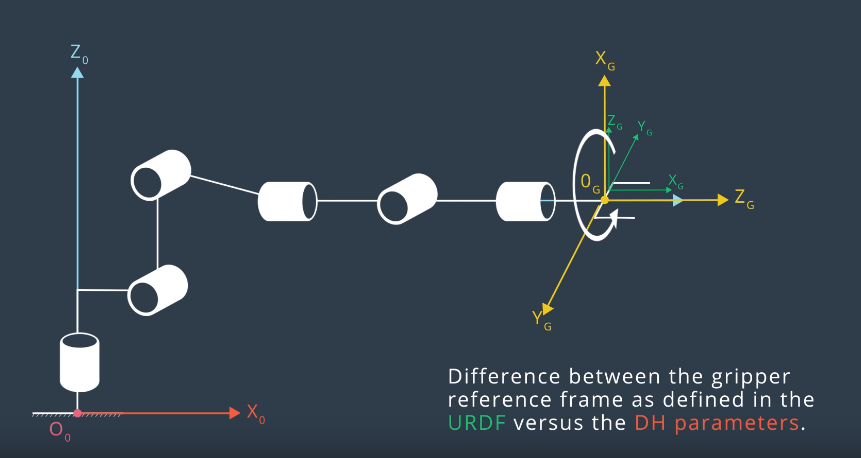
\includegraphics[width=\textwidth]{images/urdf-vs-base.png}}
\caption{Orientation of gripper frame $O_G$, URDF frame and base frame $O_0$. Screenshot from lecture 2-11.}


\label{img:urdf-vs-base}
\end{figure}

\bibliographystyle{apacite}
\bibliography{kinematics}
\end{document}  
